\documentclass[a4paper]{scrartcl}

%% Language and font encodings
\usepackage[english]{babel}
\usepackage[utf8x]{inputenc}
\usepackage[T1]{fontenc}

%% Sets page size and margins
\usepackage[a4paper,top=3cm,bottom=2cm,left=3cm,right=3cm,marginparwidth=1.75cm]{geometry}

%% Useful packages
\usepackage{amsmath}
\usepackage{graphicx}
\usepackage[colorinlistoftodos]{todonotes}
\usepackage[colorlinks=true, allcolors=blue]{hyperref}
\usepackage{placeins}
\usepackage{siunitx}
\usepackage{sidecap}
\usepackage{float}
\DeclareSIUnit\atmosphere{atm}

\title{Computed Motor Control - Lab 4}
\author{Florian Kaufmann \and Octave Martin \and Matias ???}

\begin{document}
\maketitle

\section{Introduction}
The aim of this laboratory is to model central pattern generators to simulate a primitive behaviour of a lamprey neural system. By varying the parameters, we are going to experiment different simulations to help us understand the weight of each parameter and how to modify the behavious of our lampery model.

\section{CPG model}
\subsection{Default parameters}

blabla

\begin{figure}[!h]
	\centering
	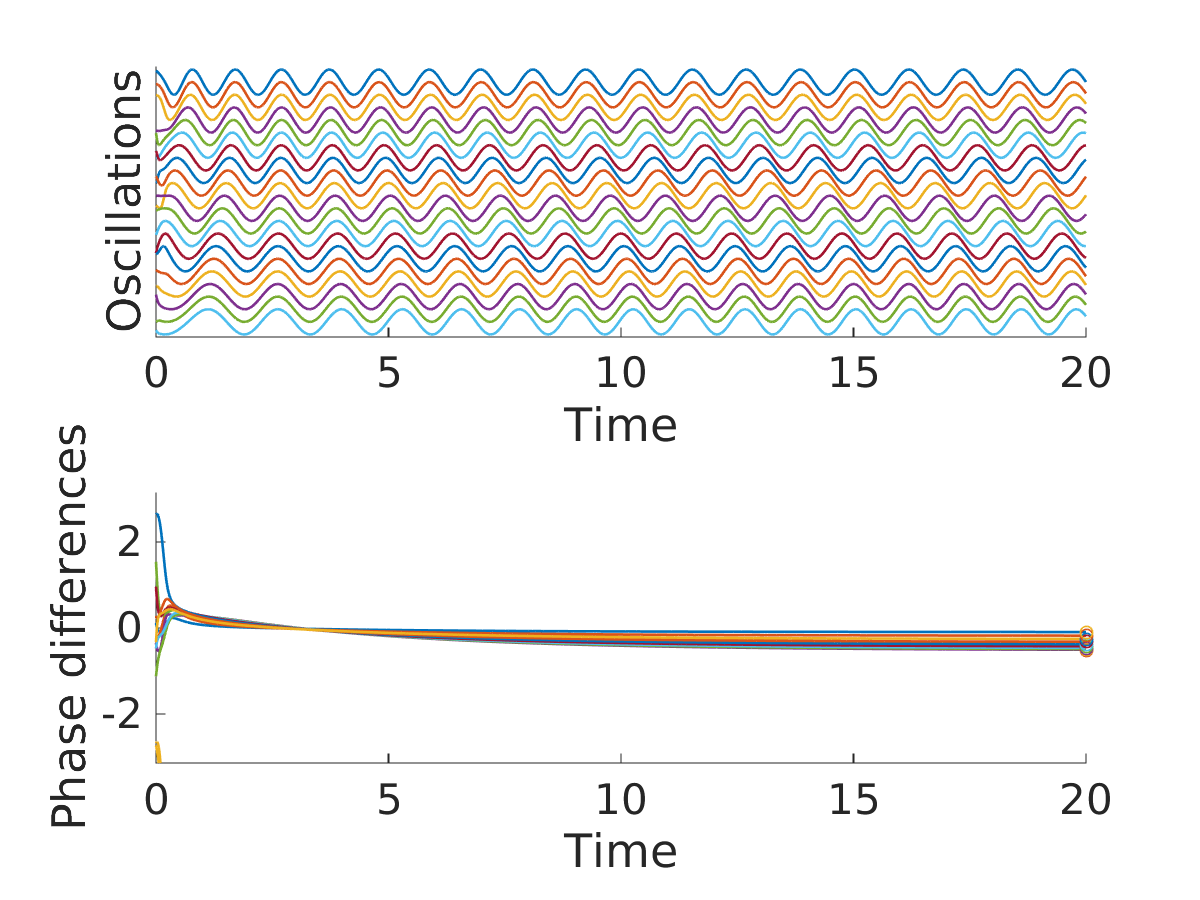
\includegraphics[width=0.5\textwidth]{fig/default1.png}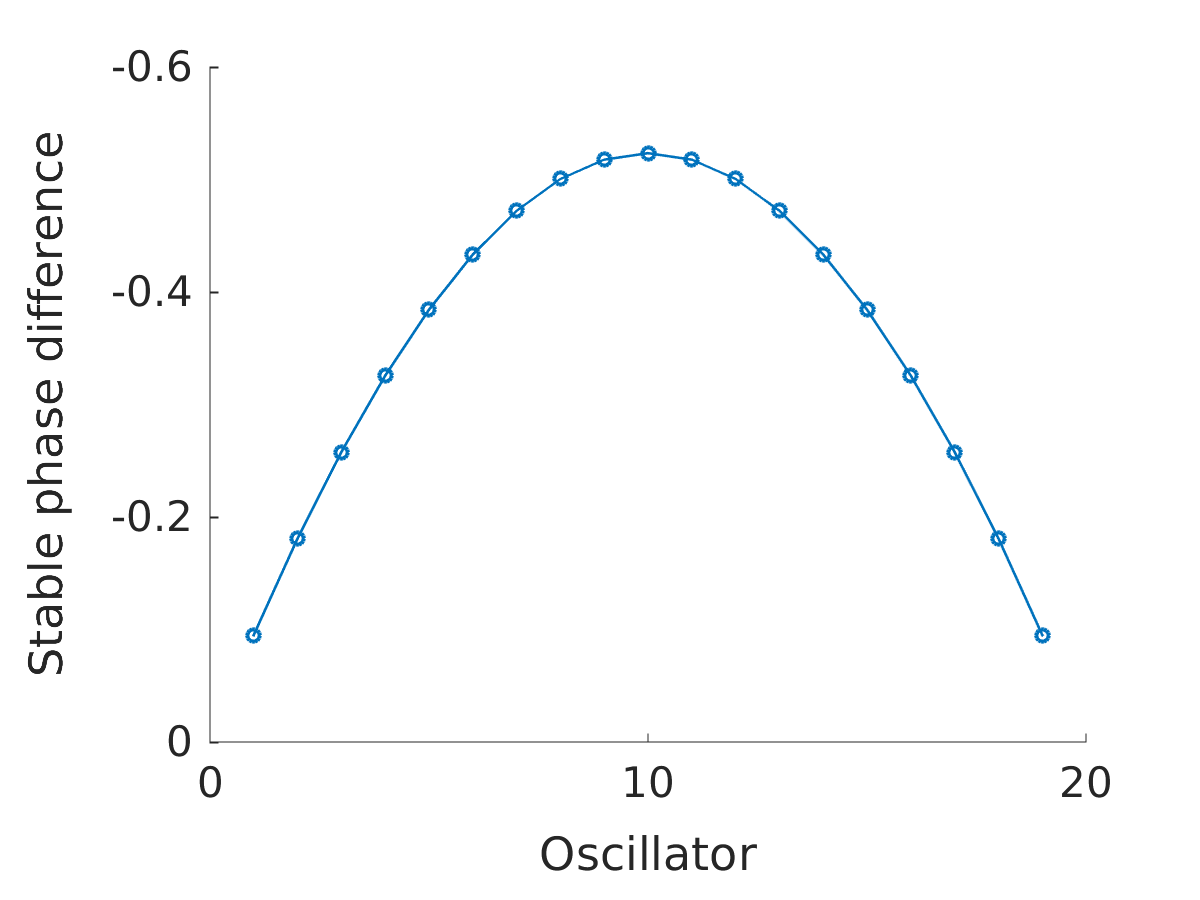
\includegraphics[width=0.5\textwidth]{fig/default2.png}
\end{figure}
\begin{SCfigure}
	\centering
	\caption{ ... caption text ...}
	\includegraphics[width=0.5\textwidth]%
	{fig/default3}% picture filename
\end{SCfigure}


\subsection{Influence of the number of oscillators}

blabla

\begin{figure}[!h]
	\centering
	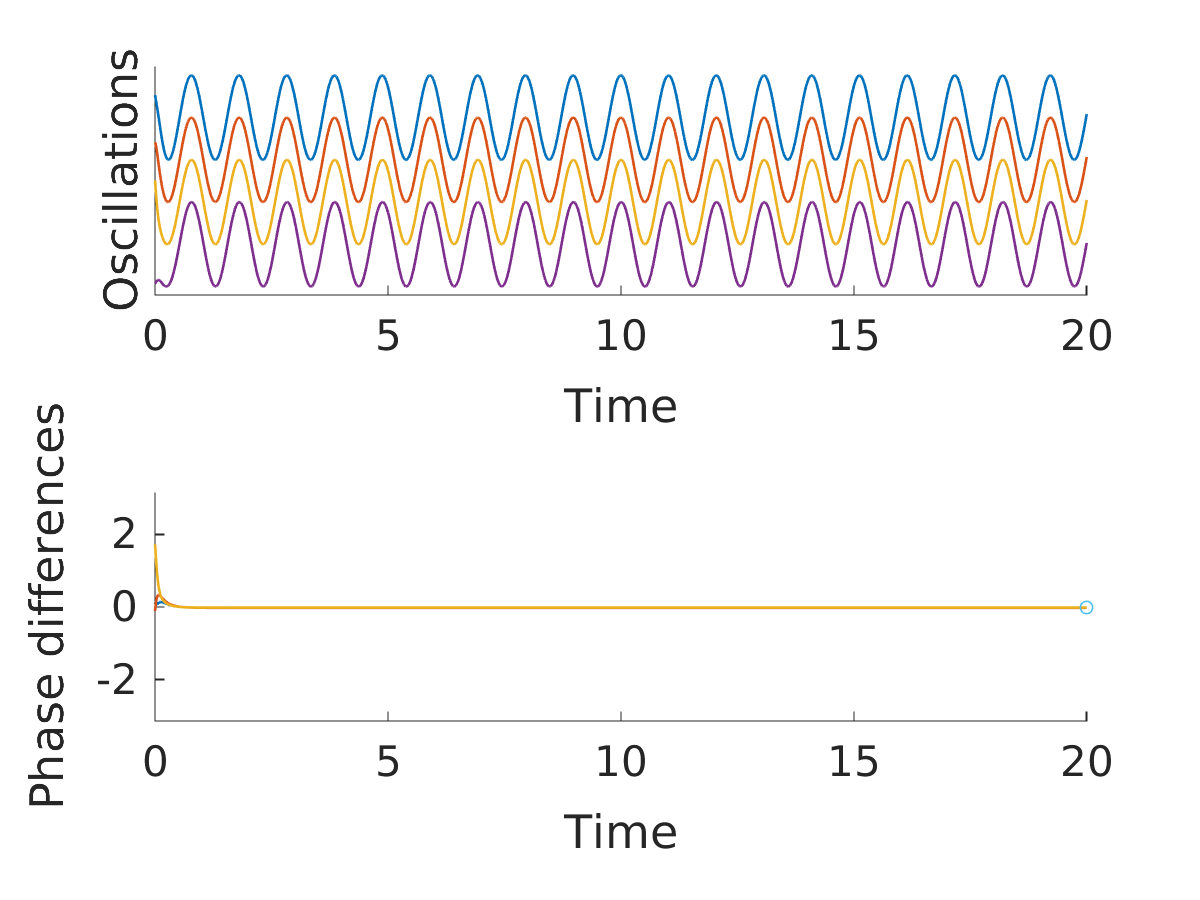
\includegraphics[width=0.5\textwidth]{fig/N1.png}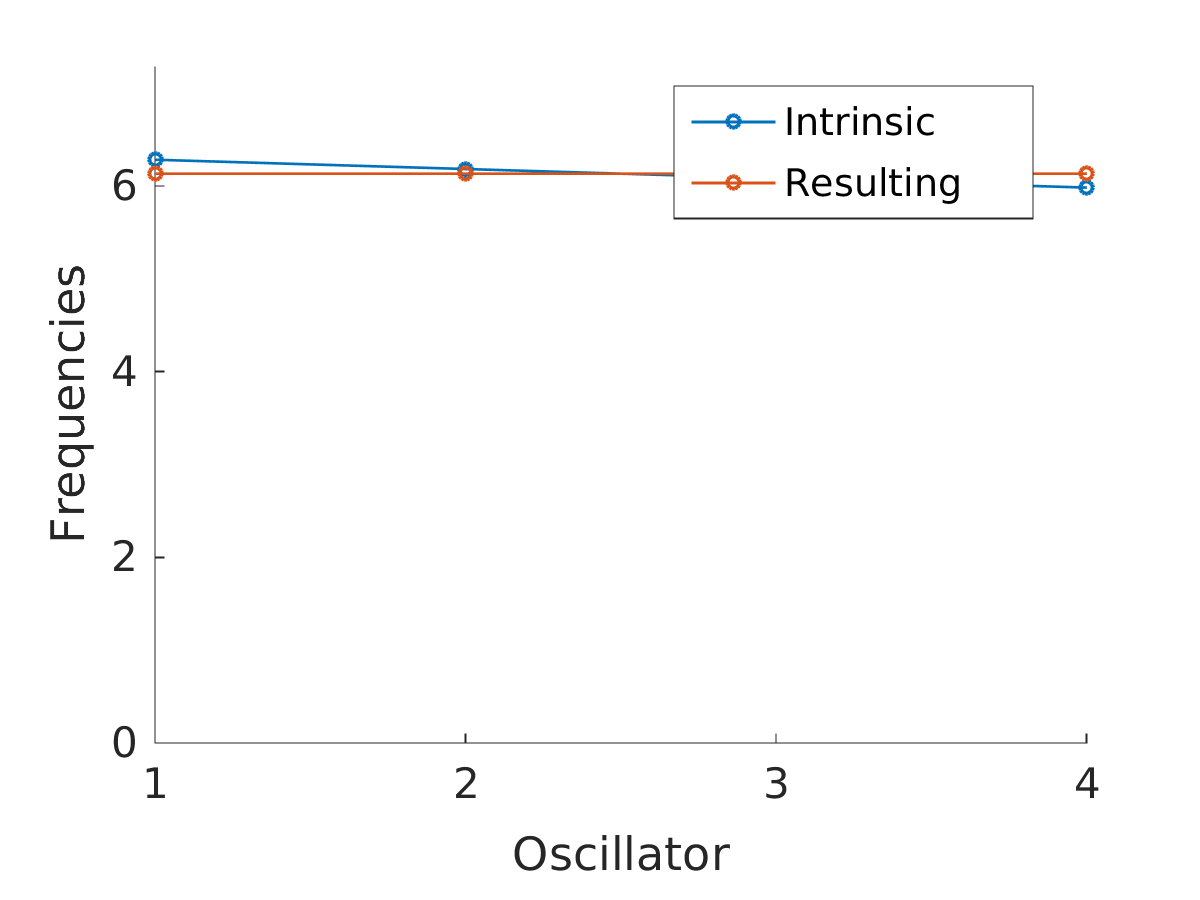
\includegraphics[width=0.5\textwidth]{fig/N2.png}
\end{figure}

\begin{SCfigure}[][h]
	\centering
	\caption{ ... caption text ...}
	\includegraphics[width=0.5\textwidth]%
	{fig/N3}% picture filename
\end{SCfigure}

\newpage
\subsection{Influence of the gradient of frequencies}

blabla..

\begin{figure}[!h]
	\centering
	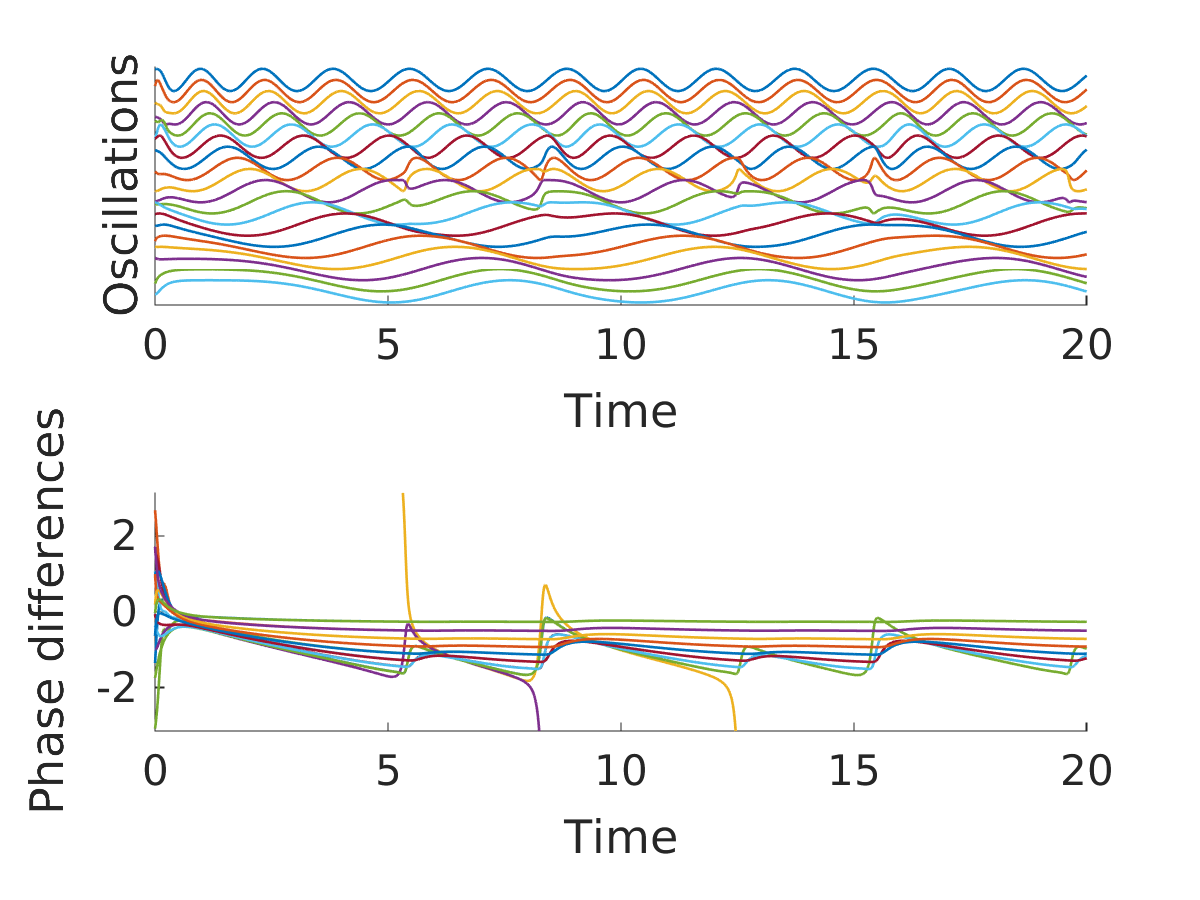
\includegraphics[width=0.5\textwidth]{fig/e1}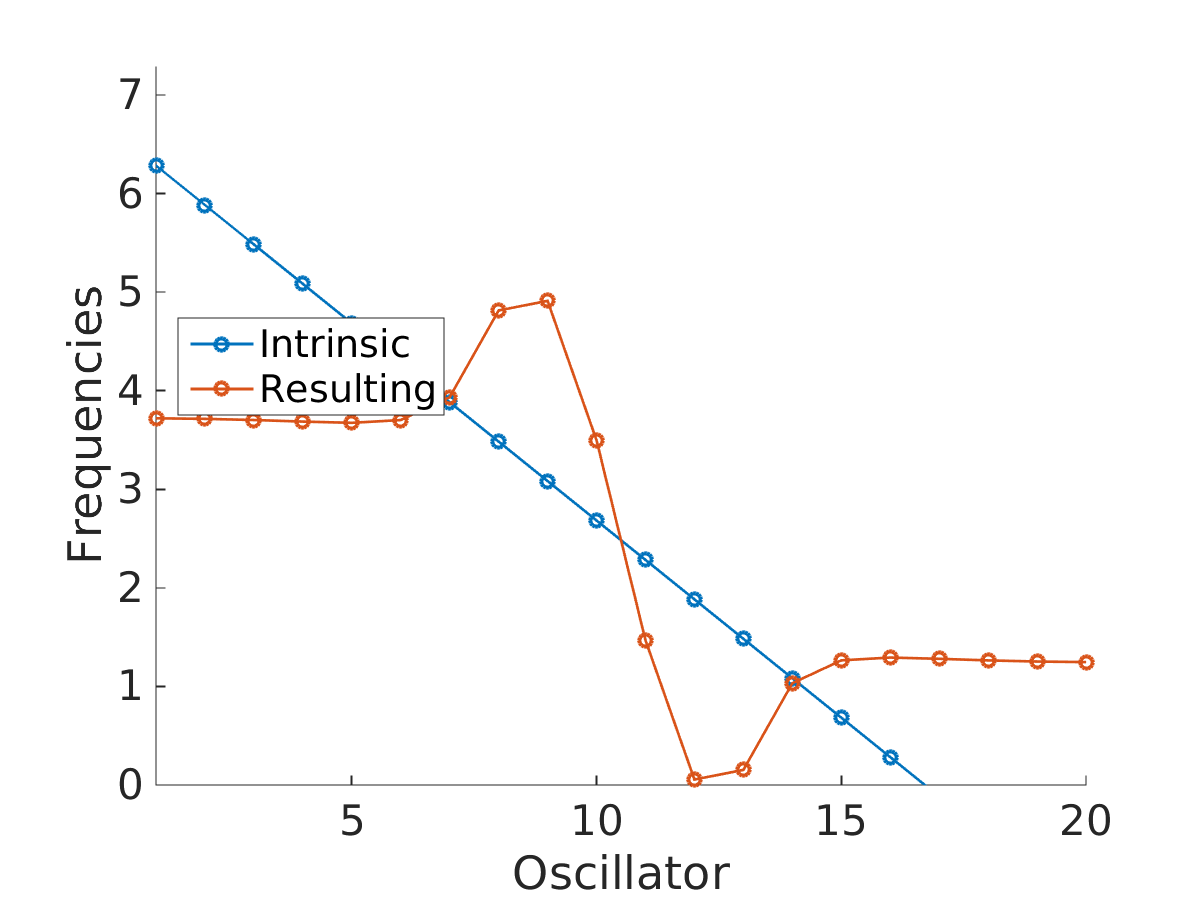
\includegraphics[width=0.5\textwidth]{fig/e2.png}
\end{figure}

\begin{SCfigure}[][h]
	\centering
	\caption{ ... caption text ...}
	\includegraphics[width=0.5\textwidth]%
	{fig/e3}% picture filename
\end{SCfigure}

\newpage
\subsection{Influence of the coupling strenght}

blabla

\subsection{Possible non linear interesting model}

blabla

\newpage
\subsection{Influence of an external load}

blabla

\begin{figure}[!h]
	\centering
	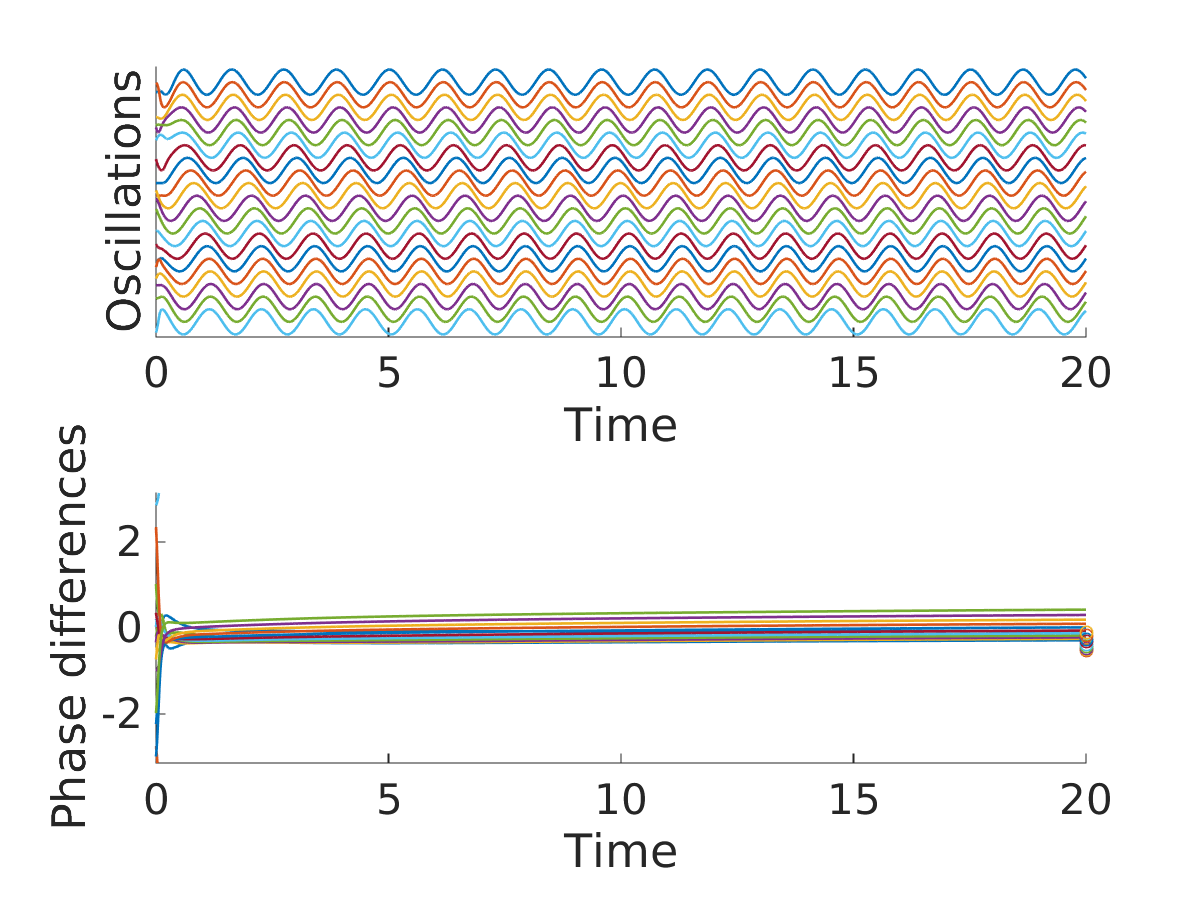
\includegraphics[width=0.5\textwidth]{fig/ext1.png}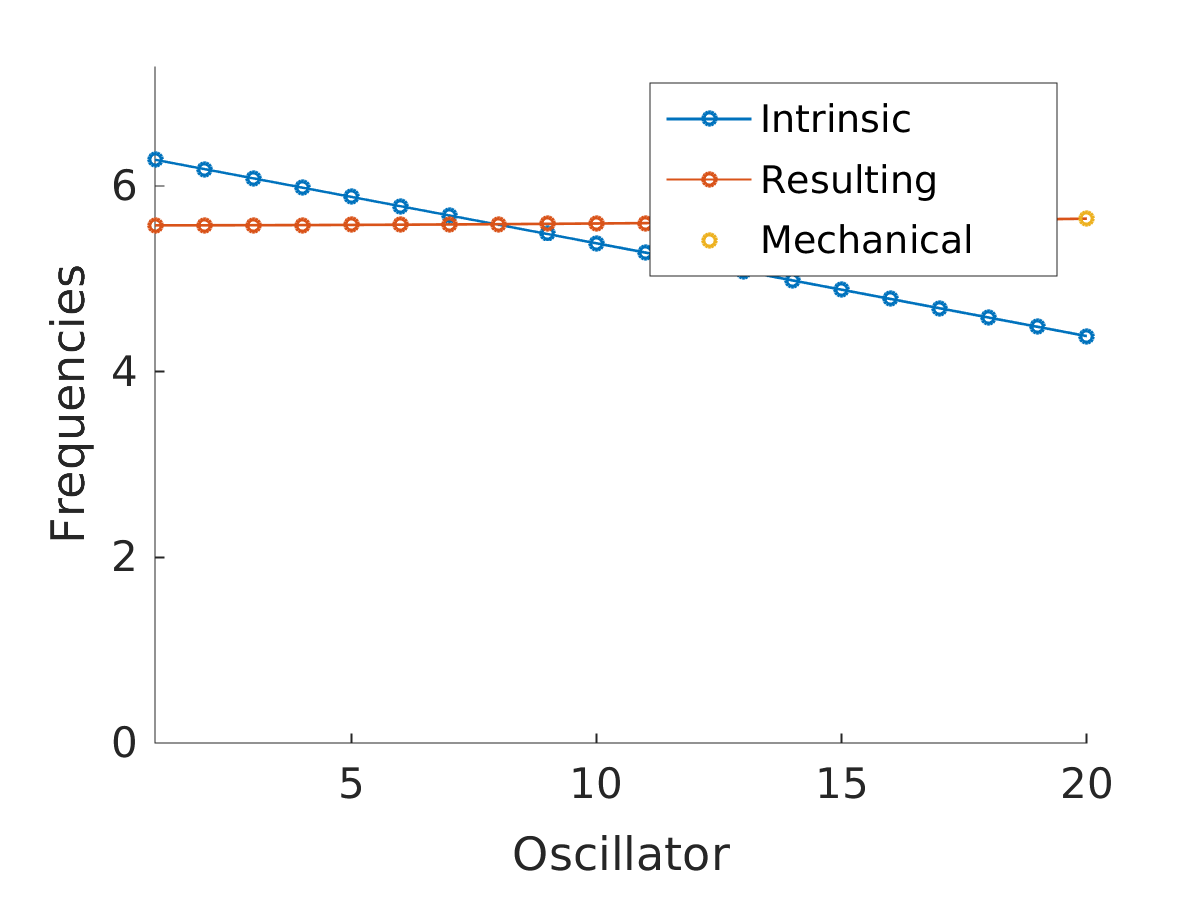
\includegraphics[width=0.5\textwidth]{fig/ext2.png}
\end{figure}

\begin{SCfigure}[][h]
	\centering
	\caption{ ... caption text ...}
	\includegraphics[width=0.5\textwidth]%
	{fig/ext3}% picture filename
\end{SCfigure}

\section{Conclusion}

blabla

\end{document}
